\subsection{Repeated source training and budget dependence}\label{app:source-replication}
We add three paired fine-tuning runs from the same pretrained FlowMol checkpoint.
Runs 3 and 5 use the first 3,000-row training block; run 4 uses the second.
Each pair shares initial weights, reference order, and optimizer settings, and
changes only the source. At 6,000 updates, the same 3,000 rows have been visited
twice. These are five stochastic fine-tuning runs on two fixed data blocks,
not five independent pretraining runs or an isolated dataset-size experiment.

Every new run is evaluated at 1,000, 3,000, and 6,000 updates on the existing
64-composition panel. The first and last checkpoints use 16 draws per composition;
the middle checkpoint uses 32, matching the original runs. All checkpoints and
all runs are reported. No checkpoint was selected using these outcomes.

\begin{table}[h]
\centering
\caption{Harmonic-minus-Gaussian graph validity in percentage points. Dashes mark
training budgets not run for the original two models.}
\begin{tabular}{lrrr}
\toprule
Fine-tuning run & 1,000 updates & 3,000 updates & 6,000 updates\\
\midrule
1 &---&$+11.18$&---\\
2 &---&$+2.64$&---\\
3 &$-1.37$&$+5.66$&$+5.96$\\
4 &$-0.10$&$+3.32$&$+3.91$\\
5 &$-3.52$&$-3.37$&$+1.95$\\
\midrule
Mean, new runs 3--5 &$-1.66$&$+1.87$&$+3.94$\\
Mean, all available runs &$-1.66$&$+3.89$&$+3.94$\\
\bottomrule
\end{tabular}
\end{table}

At 3,000 updates, the five-run mean is $+3.89$ points and the sample standard
deviation across runs is 5.27 points. The composition-bootstrap interval is
$[2.52,5.33]$, conditional on these fitted models; it does not describe uncertainty
over future training runs. For the three new runs, the corresponding intervals
are $[-4.04,0.68]$, $[0.36,3.52]$, and $[1.73,6.25]$ at the three budgets.
The source advantage depends on training duration and varies across runs.
This study adds 36,000 optimizer updates and 24,576 raw outputs, with no
physical-oracle queries.

\begin{figure}[h]
\centering
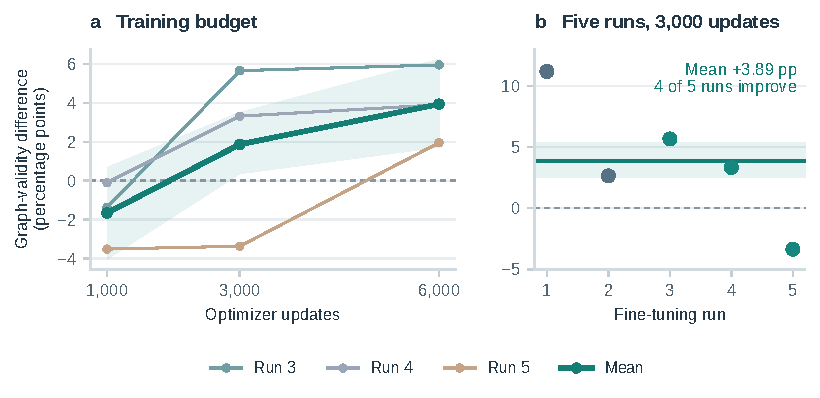
\includegraphics[width=\linewidth]{../research/figures/evidence_design_v2/source_training.pdf}
\caption{Source effects across training budgets and fine-tuning runs. Thin lines
show all three new runs; the thick line is their mean. The right panel includes
all five runs at 3,000 updates. Shading and the horizontal bar show 95\%
composition-bootstrap intervals conditional on the fitted models.}
\end{figure}
